\documentclass[12pt]{standalone}
\usepackage[utf8]{inputenc}
\usepackage[T1]{fontenc}
\usepackage{times}
\usepackage{amsmath,amssymb}
\usepackage[dvipsnames,svgnames]{xcolor}
\usepackage{tikz}
\usetikzlibrary{decorations.pathreplacing, calc, positioning, shapes.geometric, shapes.symbols, arrows.meta, backgrounds, fit, shapes.misc}
\definecolor{RED}{rgb}{1,0,0}
\definecolor{dmrsfill}{HTML}{CDE2FB}
\definecolor{winblue}{HTML}{0D366B}
\definecolor{inksec}{HTML}{52514E}
\begin{document}
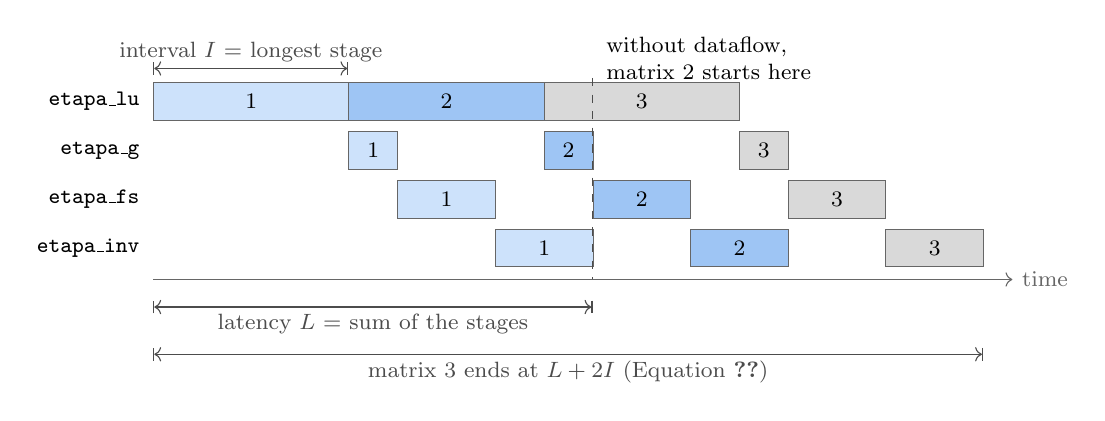
\begin{tikzpicture}[font=\fontsize{8.5}{10}\selectfont,
  tar/.style={draw=black!60, fill=#1, minimum height=0.48cm, inner sep=0pt, line width=0.3pt}]
\def\u{0.62}\def\h{0.62}
\definecolor{m1}{HTML}{CDE2FB}\definecolor{m2}{HTML}{9EC5F4}\definecolor{m3}{HTML}{D9D9D9}
% durações esquemáticas: LU = 4, G = 1, FS = 2, INV = 2 (soma 9, maior 4)
\newcommand{\caixa}[5]{% #1 linha, #2 início, #3 duração, #4 cor, #5 matriz
  \node[tar=#4, minimum width=#3*\u cm, anchor=west] at (#2*\u, -#1*\h) {#5};}
\foreach \l/\n in {0/etapa\_lu, 1/etapa\_g, 2/etapa\_fs, 3/etapa\_inv}
  \node[left, font=\fontsize{8}{9.6}\selectfont\ttfamily] at (-0.05, -\l*\h) {\n};
% matriz 1
\caixa{0}{0}{4}{m1}{1}\caixa{1}{4}{1}{m1}{1}\caixa{2}{5}{2}{m1}{1}\caixa{3}{7}{2}{m1}{1}
% matriz 2
\caixa{0}{4}{4}{m2}{2}\caixa{1}{8}{1}{m2}{2}\caixa{2}{9}{2}{m2}{2}\caixa{3}{11}{2}{m2}{2}
% matriz 3
\caixa{0}{8}{4}{m3}{3}\caixa{1}{12}{1}{m3}{3}\caixa{2}{13}{2}{m3}{3}\caixa{3}{15}{2}{m3}{3}
% eixo
\draw[black!60, ->, line width=0.4pt] (0,-3*\h-0.4) -- (17.6*\u,-3*\h-0.4) node[right] {time};
% intervalo
\draw[black!70, |<->|, line width=0.4pt] (0,0.42) -- (4*\u,0.42) node[midway, above=-1pt] {interval $I$ = longest stage};
% latência da matriz 1
\draw[black!70, |<->|, line width=0.4pt] (0,-3*\h-0.75) -- (9*\u,-3*\h-0.75) node[midway, below=-1pt] {latency $L$ = sum of the stages};
% sem dataflow
\draw[black!70, dashed, line width=0.4pt] (9*\u,0.30) -- (9*\u,-3*\h-0.4);
\node[align=left, anchor=south west] at (9*\u+0.05,0.15) {without dataflow,\\matrix 2 starts here};
% fim da matriz 3
\draw[black!70, |<->|, line width=0.4pt] (0,-3*\h-1.35) -- (17*\u,-3*\h-1.35) node[midway, below=-1pt] {matrix 3 ends at $L + 2I$ (Equation~\ref{eq:fim-tarefas})};
\end{tikzpicture}
\end{document}
